\newpage
\thispagestyle{empty}

\begin{figure}[!h]
    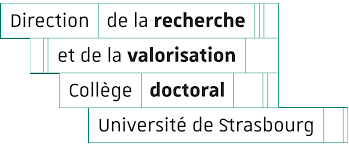
\includegraphics[width=6cm]{conformitées/figures/dir_rech.png}
\end{figure}

\center{\large{Déclaration sur l’Honneur\\[0.5cm]
                \textit{Declaration of Honour\\[0.5cm]}}}

\justify
{\setlength{\parindent}{0pt}

J’affirme être informé que le plagiat est une faute grave susceptible de mener à des sanctions administratives et disciplinaires pouvant aller jusqu’au renvoi de l’Université de Strasbourg et passible de poursuites devant les tribunaux de la République Française.\\

Je suis conscient(e) que l’absence de citation claire et transparente d’une source empruntée à un tiers (texte, idée, raisonnement ou autre création) est constitutive de plagiat.\\

Au vu de ce qui précède, j’atteste sur l’honneur que le travail décrit dans mon manuscrit de thèse est un travail original et que je n’ai pas eu recours au plagiat ou à toute autre forme de fraude.\\

\textit{I affirm that I am aware that plagiarism is a serious misconduct that may lead to administrative and disciplinary sanctions up to dismissal from the University of Strasbourg and liable to prosecution in the courts of the French Republic.\\}

\textit{I am aware that the absence of a clear and transparent citation of a source borrowed from a third party (text, idea, reasoning or other creation) is constitutive of plagiarism.\\}

\textit{In view of the foregoing, I hereby certify that the work described in my thesis manuscript is original work and that I have not resorted to plagiarism or any other form of fraud.\\[1cm]}


\textbf{Nom Prénom :} \name \\
\textbf{Ecole doctorale :} \ed \\
\textbf{Laboratoire :} \lab
}